\setcounter{chapter}{8} 
\chapter*{Chapter (8): Eye Tracking}
\addcontentsline{toc}{chapter}{Chapter (8): Eye Tracking} 
\setcounter{section}{0}

\section{Chapter Preview}
\label{sec:eye_tracking}
This chapter details the design of the webcam-based eye-tracking module developed for non-verbal or locked-in Sanad users. It outlines the camera hardware, MediaPipe face and iris landmark detection algorithms, the head-pose independent gaze vector calculation, calibration techniques, command mapping schemes, and performance evaluations.

% ----------------------------------------------------------------
\section{Camera Hardware}
% ----------------------------------------------------------------

The camera we used is EMEET C955. It works with 1920 x 1080 resolution and is connected via USB. It is mounted at the top-centre of the touchscreen bezel, angled
5--10° upward toward the user at a working distance of 35--45~cm. Frames are captured
in BGR at 30~fps and are \textbf{horizontally mirrored} immediately on read, so cursor
motion matches the user's natural gaze direction.

\begin{figure}[H]
\centering
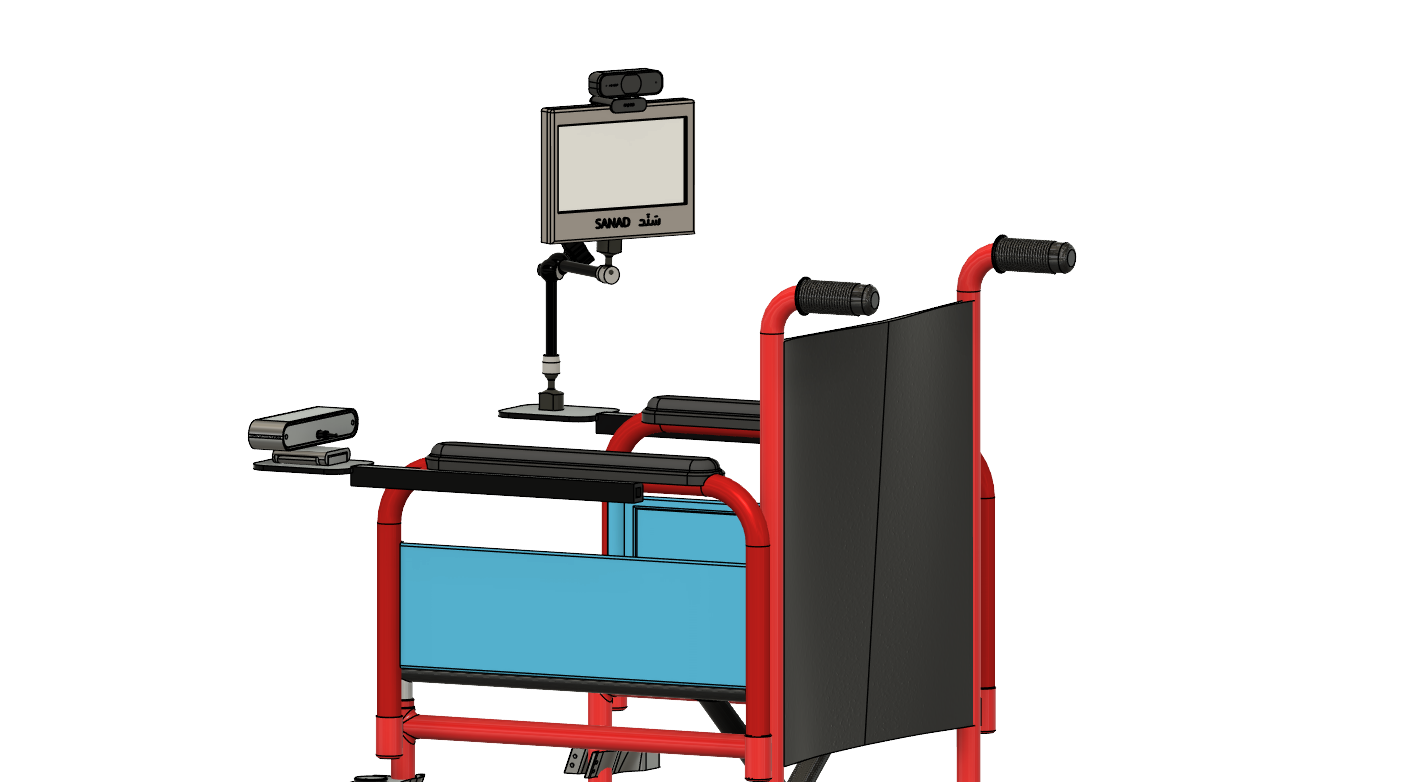
\includegraphics[width=500]{figures/ch08/20}
\label{fig:camera_hardware}
\end{figure}

\newpage

% ----------------------------------------------------------------
\subsection{Eye Tracking Algorithm: MediaPipe FaceLandmarker}
% ----------------------------------------------------------------
\subsubsection{Algorithm Selection}

Several approaches were evaluated against two criteria: real-time CPU-only performance on
the Pi~4 and accuracy sufficient for command-zone discrimination.

\begin{table}[H]
\centering
\caption{Eye Tracking Approach Comparison}
\label{tab:et_algorithm_comparison}
\begin{tabular}{p{3.5cm}p{2.0cm}p{2.5cm}p{2.0cm}p{4.0cm}}
\toprule
\textbf{Approach} & \textbf{CPU (Pi~4)} & \textbf{Accuracy} & \textbf{Decision} & \textbf{Reason} \\
\midrule
Tobii Eye Tracker 5
  & N/A (USB)   & Very High
  & Rejected & Cost ($>$\$200); proprietary SDK \\[3pt]
iTracker CNN
  & $>$90\%     & High
  & Rejected & Exceeds Pi~4 CPU budget \\[3pt]
OpenFace + dlib
  & 70--80\%    & Moderate--High
  & Rejected & Marginal remaining headroom \\[3pt]
GazeTracking (pupil)
  & 20--30\%    & Low--Moderate
  & Rejected & No iris model; poor low-light \\[3pt]
\textbf{MediaPipe FaceLandmarker}
  & \textbf{30--45\%} & \textbf{Moderate--High}
  & \textbf{Selected} & \textbf{Reasonable accuracy with suitable computational load} \\
\bottomrule
\end{tabular}
\end{table}

\textbf{MediaPipe FaceLandmarker} (Tasks API, \texttt{mediapipe} $\geq$ 0.10) was selected
as the optimal trade-off between accuracy and embedded performance. It ships a
float16-quantised TFLite model (\texttt{face\_landmarker.task}, $\approx$3.6~MB) that
produces \textbf{478 facial landmarks} — including a dedicated iris sub-model — at 20--28~fps
on the Pi~4 CPU without GPU. The model runs in \textbf{VIDEO mode}, feeding each frame with
a monotonically increasing timestamp so the tracker exploits temporal context across frames
for improved stability.

\begin{figure}[H]
\centering
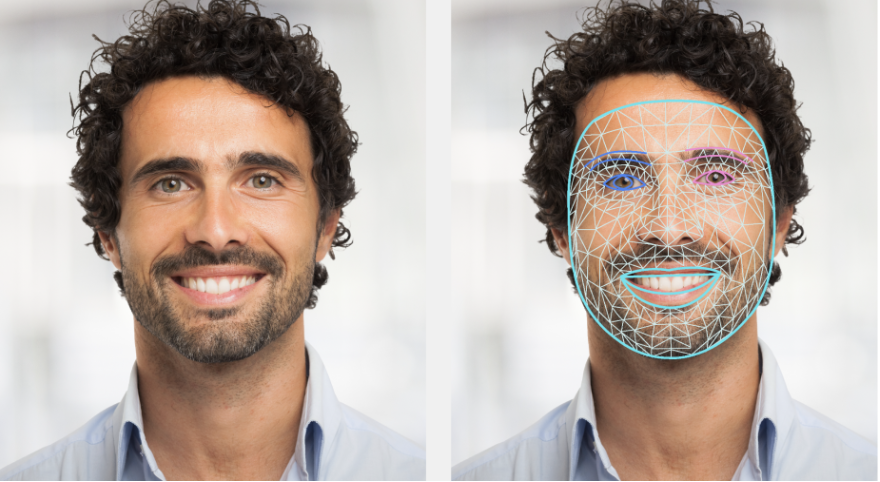
\includegraphics[width=300]{figures/ch08/fig2_latex.png}
\label{fig:mediapipe_face_landmark}
\end{figure}

\subsection{Iris Landmark Indices}

The iris centre is computed as the centroid of four
boundary landmarks per eye (indices 469–472 for the left eye, 474–477 for
the right). Its position is expressed as a fraction of the eye's own width
using the inner and outer eye corners (indices 33/133 and 362/263) as the
reference frame, making the measurement inherently robust to small head
translations.

\begin{table}[h!]
\centering
\caption{MediaPipe Landmark Indices Used by the Eye Tracking Pipeline}
\label{tab:et_landmarks}
\begin{tabular}{lll}
\toprule
\textbf{Landmark Group} & \textbf{Indices} & \textbf{Usage} \\
\midrule
Left iris boundary      & 469, 470, 471, 472      & Gaze X/Y (user's right eye) \\
Right iris boundary     & 474, 475, 476, 477      & Gaze X/Y (user's left eye) \\
Left eye corners        & 33 (inner), 133 (outer) & Horizontal normalisation \\
Right eye corners       & 362 (inner), 263 (outer) & Horizontal normalisation \\
Left eyelid top/bottom  & 159 / 145               & EAR blink detection \\
Right eyelid top/bottom & 386 / 374               & EAR blink detection \\
\bottomrule
\end{tabular}
\end{table}

\begin{figure}[H]
\centering
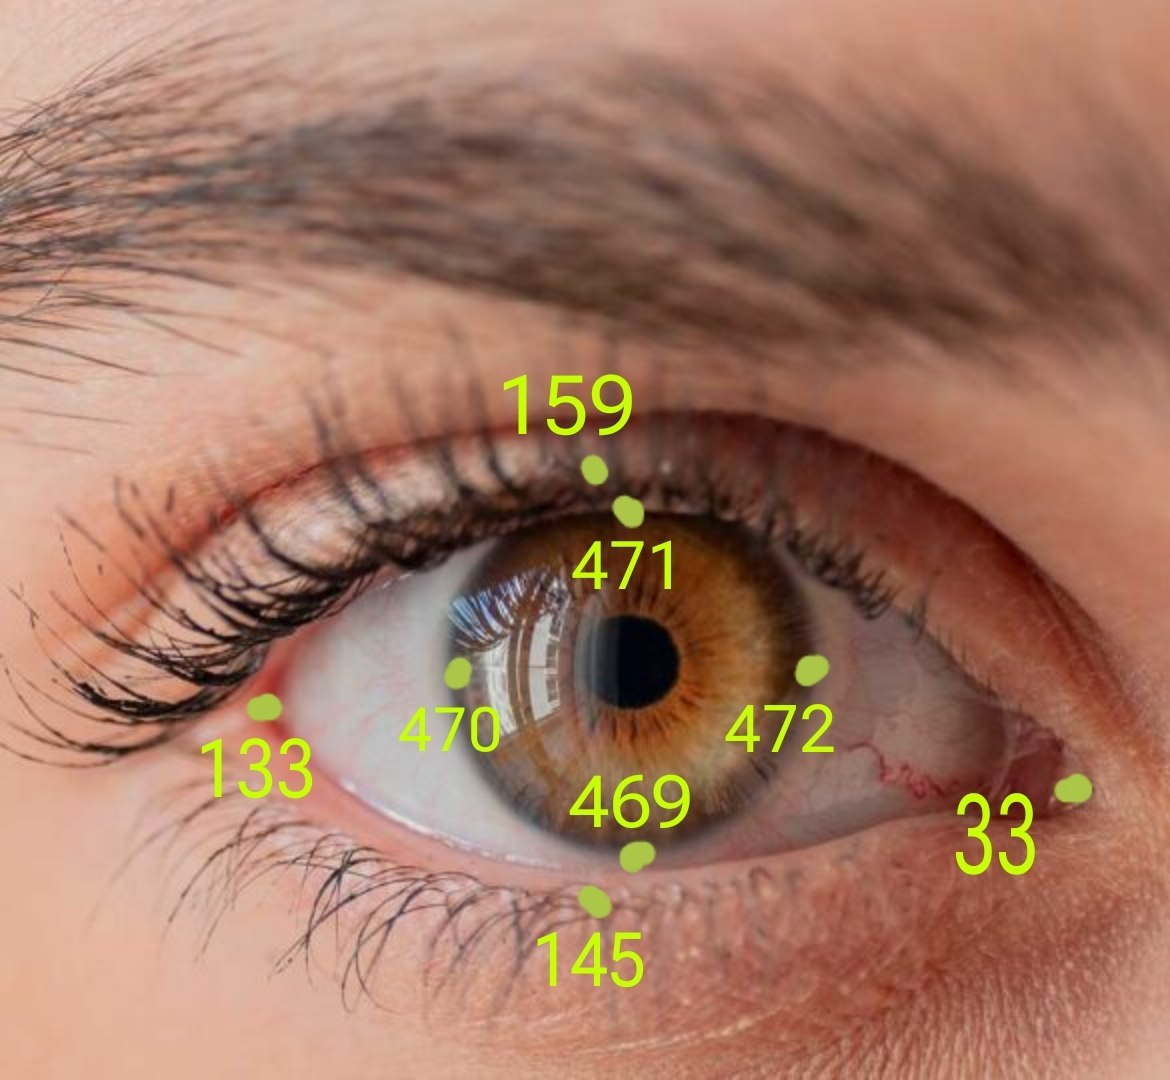
\includegraphics[width=300]{figures/ch08/fig3_latex}
\label{fig:iris_indicies}
\end{figure}

% ----------------------------------------------------------------
\section{Gaze Vector Computation: Iris Ratio Method}
% ----------------------------------------------------------------

The gaze position is computed using the \textbf{Iris Ratio Method}, which expresses the
iris location as a fraction of the eye's own extent. This makes the measurement inherently
insensitive to small head translations.

\textbf{Step 1 — Iris centre:} The four boundary landmarks per eye are averaged to pixel
coordinates $(x_c, y_c)$. Both eyes are averaged to reduce single-eye occlusion noise.

\begin{equation}
    x_c = \frac{1}{4} \sum_{k \in \mathcal{I}} \lambda_k^x \cdot W, \qquad
    y_c = \frac{1}{4} \sum_{k \in \mathcal{I}} \lambda_k^y \cdot H
    \label{eq:iris_centre}
\end{equation}

\textbf{Step 2 — Iris ratio:} The iris displacement within the eye socket is expressed as a
normalised ratio, where $x_L, x_R$ are the eye corner $x$-coordinates, $y_M$ is the
vertical eye midline, and $w_e = x_R - x_L$ is the eye width:

\begin{align}
    r_h &= \frac{x_c - x_L}{w_e} - 0.5, \qquad
    r_v  = \frac{y_c - y_M}{w_e}
    \label{eq:ratios}
\end{align}

\textbf{Step 3 — Normalisation:} Per-user offset ($\delta$) and range ($\rho$) calibration
parameters are applied:
$\hat{r} = (r - \delta) / \rho$.

\textbf{Step 4 — Non-linear power curve:} A signed power-law sharpens central precision
while preserving full edge access:

\begin{equation}
    \tilde{r} = \operatorname{sign}(\hat{r}) \cdot |\hat{r}|^{1.2}
    \label{eq:power_curve}
\end{equation}

\textbf{Step 5 — Screen mapping:} The result is clamped and remapped to $[0, 1]$: \newline
$g = \bigl(\operatorname{clip}(\tilde{r}, -1, 1) + 1\bigr) / 2$.
The final pair $(g_x, g_y)$ is published on \newline \texttt{/eye\_tracking/gaze\_position} at 30~Hz.

% ----------------------------------------------------------------
\section{Blink Detection and Temporal Filtering}
% ----------------------------------------------------------------

\textbf{Eye Aspect Ratio (EAR):} Blink and eye-closure events are detected using the
EAR metric, defined as the ratio of vertical eye opening to horizontal
eye span. Open eyes yield EAR $\approx 0.28$--$0.35$; a closed eye drops below the
threshold $\theta_{\text{EAR}} = 0.20$.

\begin{equation}
    \text{EAR} = \frac{\| \mathbf{p}_{\text{top}} - \mathbf{p}_{\text{bottom}} \|}
                      {\| \mathbf{p}_{\text{left}} - \mathbf{p}_{\text{right}} \|}
    \label{eq:ear}
\end{equation}

The eye state published on \texttt{/eye\_tracking/eye\_state} is \texttt{"open"} when
$\text{EAR} \geq \theta$, \texttt{"blink"} on the first frame of closure, and
\texttt{"closed"} on sustained closure.

\textbf{EMA smoothing:} Raw iris positions are smoothed by an Exponential Moving Average
applied only during open-eye frames to suppress micro-saccade jitter:

\begin{equation}
    \hat{g}_t = \alpha \cdot g_t + (1 - \alpha)\cdot\hat{g}_{t-1}, \qquad \alpha = 0.30
    \label{eq:ema}
\end{equation}

On blink or closure, the EMA update freezes and the last valid position is held.

\textbf{Blink-rewind buffer:} During a natural blink the upper eyelid physically pushes
the iris downward before closure, which would otherwise shift the cursor toward the screen
bottom on every blink. A \textbf{circular history buffer}
(\texttt{deque(maxlen=7)}, $\approx$230~ms) stores recent open-eye gaze positions.
On blink detection, the cursor is rewound to the oldest buffer entry — the pre-blink gaze
state — making blinks completely transparent to cursor position.

% ----------------------------------------------------------------
\section{Calibration}
% ----------------------------------------------------------------

Calibration is performed by adjusting per-user parameters in \newline
\texttt{config/eye\_tracking\_params.yaml}. With the debug overlay enabled, the user
looks at screen centre to set offsets, then at the edges to set range; the full procedure
takes under two minutes and the profile is saved for reuse.

\begin{table}[H]
\centering
\caption{Eye Tracking Key Configuration Parameters}
\label{tab:et_calib_params}
\begin{tabular}{lll}
\toprule
\textbf{Parameter} & \textbf{Default} & \textbf{Description} \\
\midrule
\texttt{gaze\_range\_horizontal} & 0.040   & Max horizontal iris displacement \\
\texttt{gaze\_range\_vertical}   & 0.020   & Max vertical iris displacement \\
\texttt{gaze\_offset\_horizontal}& 0.000   & Resting-gaze horizontal zero-point \\
\texttt{gaze\_offset\_vertical}  & $-$0.015 & Resting-gaze vertical zero-point \\
\texttt{gaze\_smoothing}         & 0.30    & EMA factor $\alpha$ (lower = smoother, laggier) \\
\texttt{ear\_threshold}          & 0.20    & EAR closure threshold \\
\texttt{click\_hold\_time}       & 2.0\,s  & Sustained closure duration to emit a click \\
\texttt{command\_cooldown}       & 1.0\,s  & Minimum interval between commands \\
\bottomrule
\end{tabular}
\end{table}

% ----------------------------------------------------------------
\section{Gaze-to-Command Mapping: Design Iterations}
% ----------------------------------------------------------------

Translating raw gaze data into wheelchair commands is the most user-facing design challenge
in the eye tracking module. Because Sanad targets users with severe or total loss of motor
function, every candidate mechanism must work with \textit{zero} reliance on hands, fingers,
or deliberate physical movement. The team evaluated four distinct interaction paradigms in
sequence, each informing the next, before arriving at the final design. The following
subsections document each iteration — its rationale, prototype, observed failure modes, and
the reasons it was either rejected or carried forward.

% ......................................
\subsection{Iteration 1 — Hand Gesture Control (Rejected)}
% ......................................

The first candidate explored was \textbf{hand gesture recognition} using the camera feed.
Gestures such as a raised palm, pointing finger, or directional swipe would be mapped to
navigation commands. This approach is computationally mature and widely used in consumer
devices.

However, it was rejected immediately after reviewing the primary user profile. ALS patients
— the core target population — lose voluntary muscle control progressively, with upper-limb
paralysis typically preceding or concurrent with the need for a powered wheelchair.
Requiring any deliberate hand or arm movement directly contradicts the accessibility
objective of the module. No prototype was built for this iteration.

% ......................................
\subsection{Iteration 2 — Blink-Coded Commands (Rejected)}
% ......................................

The second design attempted to repurpose natural eye closure as a \textbf{morse-code-like
input channel}. Different blink sequences were mapped to different commands: for example,
two rapid blinks triggered a \textit{right} movement, three rapid blinks triggered
\textit{left}, a sustained 3-second eye closure confirmed a selection, and other patterns
encoded \textit{forward}, \textit{backward}, and \textit{back/cancel}. The appeal of this
system was that it required only the eyes — no gaze tracking hardware beyond a webcam — and
could in principle provide a rich enough vocabulary to cover all necessary commands.

A prototype was built and tested. The following failure modes were observed:

\begin{itemize}
    \item \textbf{High false-positive rate:} A healthy person blinks involuntarily 15--20
    times per minute. Every natural blink was a potential accidental command. The system
    struggled fundamentally to distinguish an intentional ``two-blink right'' sequence from
    a natural blink followed by a second natural blink a fraction of a second later. Tuning
    the inter-blink timing threshold was a losing battle: tightening it caused missed
    intentional commands; loosening it caused more false triggers.

    \item \textbf{Severe eye fatigue:} Performing deliberate, counted blink sequences
    continuously throughout a navigation session required constant conscious effort from the
    user. Testers reported eye strain and dry eyes within minutes, as blinking was no longer
    a reflexive, restful action but a deliberate, repetitive one.

    \item \textbf{Cognitive load:} Memorising and executing the correct blink count for each
    command (especially under time pressure, e.g. approaching an obstacle) added significant
    mental effort on top of the already demanding task of navigating.
\end{itemize}

This iteration was rejected. The fundamental problem was that it treated the same physiological
signal — a blink — as both noise (natural blinks) and signal (intentional commands), with no
reliable way to separate them.

% ......................................
\subection{Iteration 3 — Five-Zone Frame Division (Rejected)}
% ......................................

The third design shifted to a purely \textbf{gaze-based dwell system}, eliminating blink
counting entirely. The screen was divided into five regions by drawing both diagonals of the
display rectangle: the resulting four triangular regions pointed up, down, left, and right
respectively, with a fifth rectangular zone at the centre of the screen. The user would navigate
by dwelling — holding their gaze still — inside one of the four directional triangles for a
fixed dwell time (3 seconds), which sent a single movement step in that direction. Dwelling
at the centre triggered a \textit{click/select} action. Sustained eye closure (3 seconds)
was retained as the \textit{back/cancel} command, since no screen zone could comfortably
serve that role without conflicting with navigation.

\begin{figure}[H]
\centering
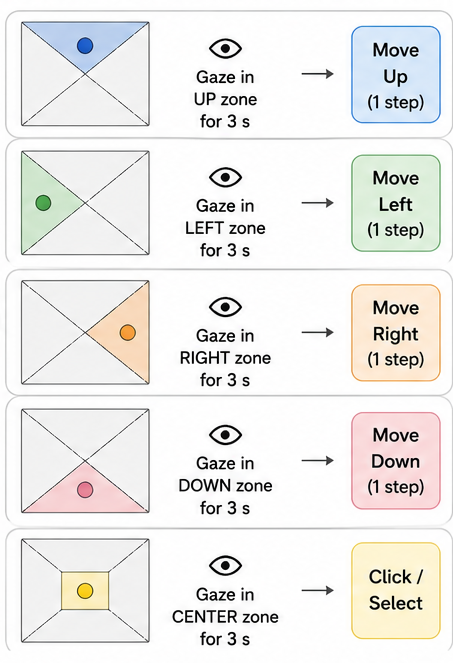
\includegraphics[width=200]{figures/ch08/fig4_latex.png}
\label{fig:system3}
\end{figure}

\newpage

This system was a significant improvement over Iteration~2 in two respects:

\begin{itemize}
    \item \textbf{Dramatic reduction in false positives:} Natural blinks had no effect
    whatsoever, as the system only measured sustained gaze position, not eye closure events.
    \item \textbf{Reduced fatigue:} Users no longer needed to consciously count or time
    blinks. Simply looking in a direction was enough.
\end{itemize}

However, two new failure modes emerged:

\begin{itemize}
    \item \textbf{Dwell-while-reading false triggers:} Users frequently dwell in a screen
    region for more than 3 seconds simply because they are \textit{reading} content in that
    area of the display. A user reading text in the lower-right of the screen would
    inadvertently trigger a \textit{right} or \textit{down} movement while doing nothing
    other than reading. This produced unexpected motion and was disorienting.

    \item \textbf{Low throughput for compound actions:} Executing any non-trivial task
    required many sequential dwell steps. For instance, navigating from the home screen to
    a specific destination required multiple \textit{right}/\textit{down} steps, each
    costing at least 3 seconds of deliberate gaze. Complex actions became slow and tiring.
\end{itemize}

The five-zone system was rejected, but its core insight — that dwell-based selection is
far superior to blink counting for ALS users — was carried into the fourth iteration.

% ......................................
\subection{Iteration 4 — Edge-Popup Dwell Buttons (Selected)}
% ......................................

The fourth and final design retained dwell-based selection but fundamentally restructured
how commands are presented and triggered. Instead of dividing the entire screen into
navigation zones (which conflicted with reading), \textbf{eight action buttons} are placed
at the edges and corners of the screen — invisible during normal use and appearing only when
the user's gaze deliberately approaches the screen periphery (within 18\% of any edge).

\begin{figure}[H]
\centering
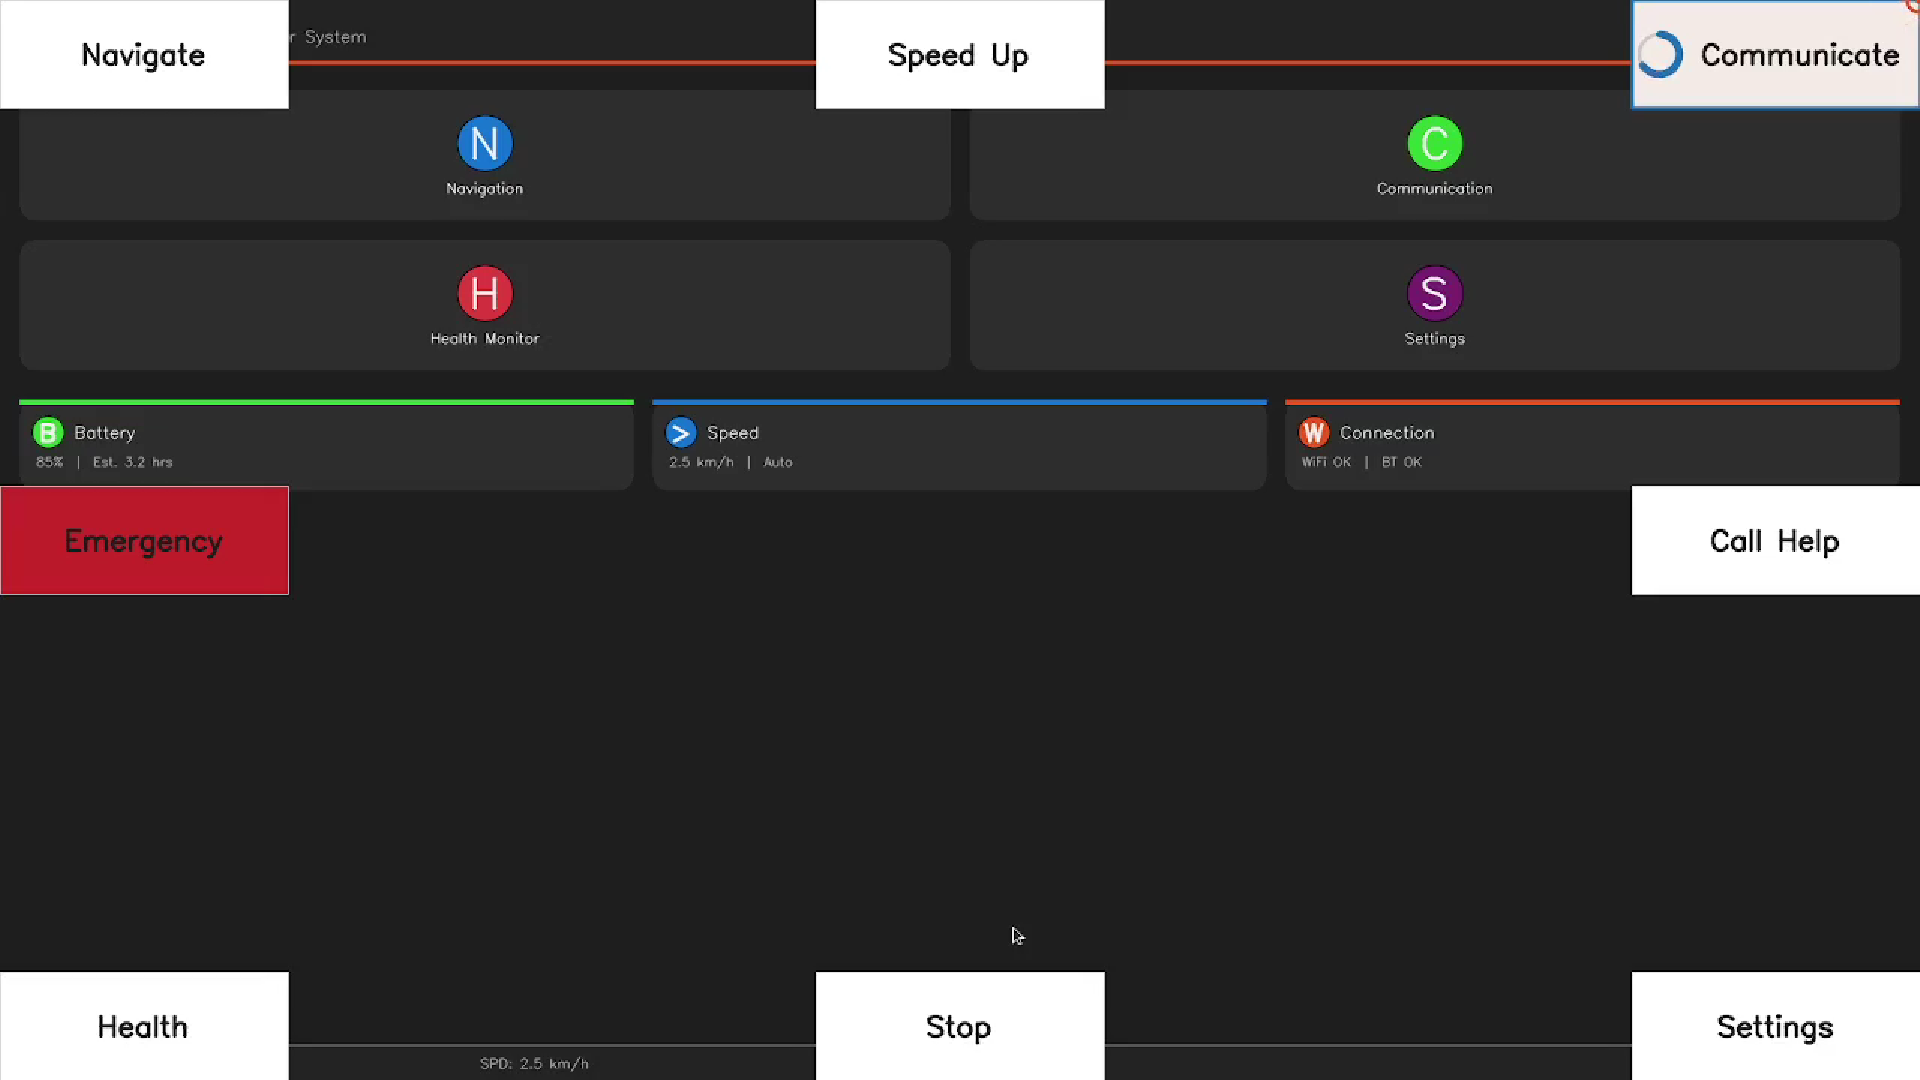
\includegraphics[width=450]{figures/ch08/fig6_latex.png}
\label{fig:system4}
\end{figure}

\begin{figure}[H]
\centering
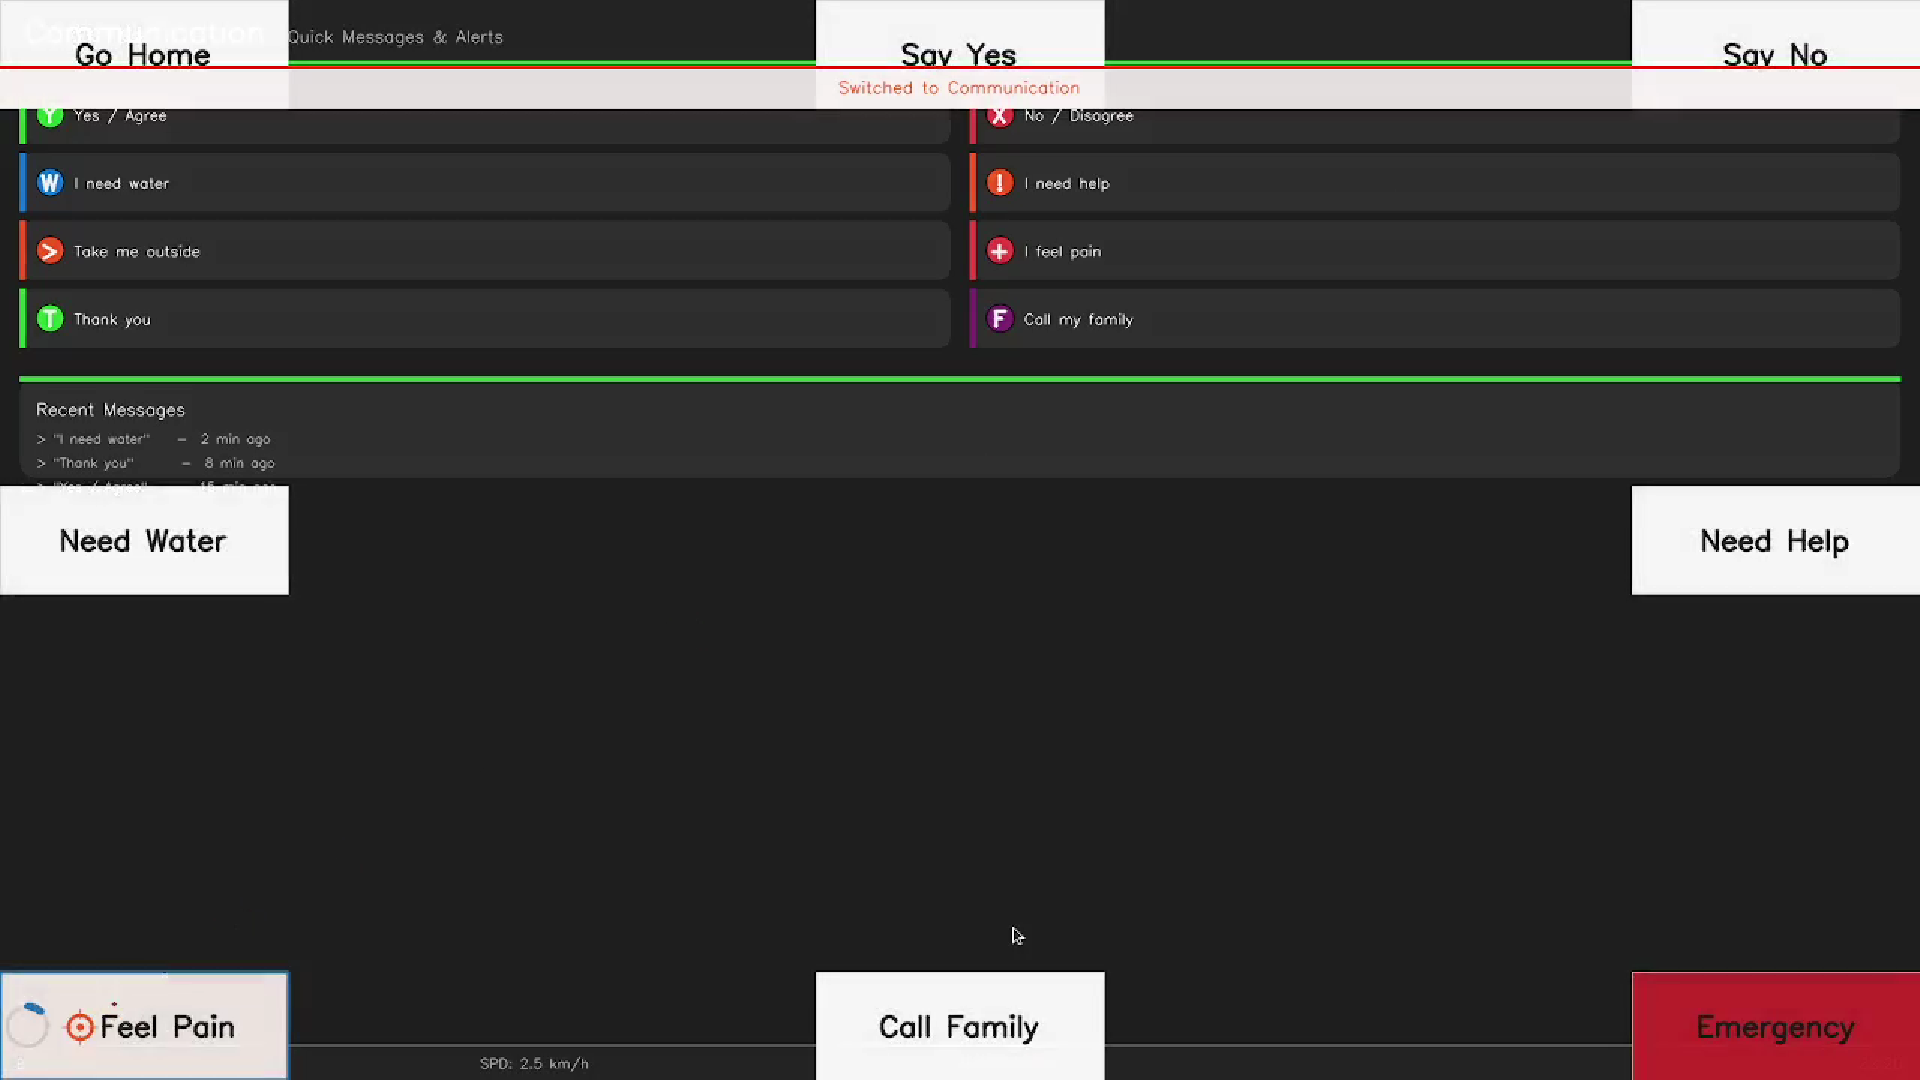
\includegraphics[width=450]{figures/ch08/fig7_latex.png}
\caption{The Selected Gaze Command Control system in action.}
\label{fig:system4_1}
\end{figure}

This design addressed both failure modes from Iteration~3:

\begin{itemize}
    \item \textbf{No false triggers while reading:} The central 82\% of the screen contains
    no interactive elements. A user reading content anywhere in that area cannot accidentally
    trigger a command regardless of how long they dwell there.

    \item \textbf{Context-sensitive actions:} Each of the  application screens (Home,
    Navigation, Communication, Health Monitor, Settings, ...etc) defines its own set of eight button
    labels. The most crucial seven actions for that specific screen are always one dwell
    away, dramatically reducing the number of steps needed per task compared to
    Iteration~3's sequential navigation model.

    \item \textbf{Reduced dwell time:} Because each button maps directly to a meaningful
    action rather than a single step, the dwell threshold reduced from 3 to 2 seconds
    without increasing false positives, making the interface 33.33 percent  faster.
\end{itemize}
When gaze enters the edge zone, the corresponding buttons fade in smoothly (4--5 frame
transition at 30~fps). During a dwell, a \textbf{progress slider} sweeps around the
button from start to end of the button, giving the user continuous visual feedback of progress toward
activation. A 0.6~s cooldown after each activation prevents unintended double-firing.
Sustained eye closure ($\geq$~2.0~s) is preserved as a universal \textit{back/cancel}
command across all screens, handled by the \texttt{gaze\_controller\_node}.

% ......................................
\subection{Interaction Design Comparison Summary}
% ......................................

Table~\ref{tab:et_interaction_comparison} summarises all four iterations across the
key evaluation criteria used to guide each design decision.

\begin{table}[H]
\centering
\caption{Gaze Interaction Design Iteration Comparison}
\label{tab:et_interaction_comparison}
\begin{tabular}{p{2.8cm}p{3.2cm}p{2.6cm}p{3.2cm}p{1.6cm}}
\toprule
\textbf{System} & \textbf{Mechanism} & \textbf{Advantages} & \textbf{Failure Mode} & \textbf{Decision} \\
\midrule
Iteration 1 \newline Hand Gestures
  & Camera-based gesture recognition
  & Mature technology; rich vocabulary
  & Requires functioning hands; incompatible with ALS target users
  & Rejected \\[6pt]

Iteration 2 \newline Blink-Coded
  & Blink count sequences (e.g.\ 2 blinks = right, 3 = left, 3\,s closure = confirm)
  & Eyes-only; no gaze tracking required
  & Severe false positives from natural blinks; eye fatigue; dry eyes; high cognitive load
  & Rejected \\[6pt]

Iteration 3 \newline Five-Zone Frame
  & Screen divided into 5 dwell regions via diagonals; 3\,s dwell per step; 3\,s closure = back
  & No blink false positives; low fatigue
  & False triggers while reading; low throughput (many steps per task)
  & Rejected \\[6pt]

\textbf{Iteration 4} \newline \textbf{Edge-Popup Dwell}
  & 8 context-sensitive buttons at screen edges; appear only when gaze nears periphery; 3\,s closure = back
  & \textbf{No false triggers while reading; context-sensitive actions; reduced dwell time; fast task completion}
  & Requires accurate gaze to reach edges reliably
  & \textbf{Selected} \\
\bottomrule
\end{tabular}
\end{table}

% ......................................
\subsection{Final Implementation: ROS 2 Command Node}
% ......................................
The \texttt{gaze\_controller\_node} subscribes to \texttt{/eye\_tracking/eye\_state} and
    implements a three-state machine to handle the eye-closure back command. 
    \begin{itemize}
        \item While the eye is
        \texttt{"open"}, the cursor tracks the live gaze position. 
        \item A \texttt{"blink"} event freezes
        the cursor and resets the closure timer. 
        \item Sustained \texttt{"closed"} state for
        $\geq$~2.0~s emits a \texttt{"click"} command on \texttt{/eye\_tracking/command}, followed
        by a 0.6~s cooldown to prevent repeat triggers. 
\end{itemize}
This mechanism handles back/cancel and
confirm actions at the system level, while all directional and screen-specific actions are handled by the edge-popup dwell system in the touchscreen UI layer.

% ----------------------------------------------------------------
\section{Gaze Pipeline Diagram}
% ----------------------------------------------------------------
The eye-tracking pipeline is divided into two ROS 2 nodes. The eye\_tracker\_node acquires camera frames, estimates the user's gaze using MediaPipe and iris-based processing, and publishes the gaze position and eye state. The gaze\_controller\_node subscribes to these topics, executes the command state machine to interpret user intent (tracking, blink, or sustained eye closure), and generates the corresponding control commands for the wheelchair.

\begin{figure}[H]
\centering
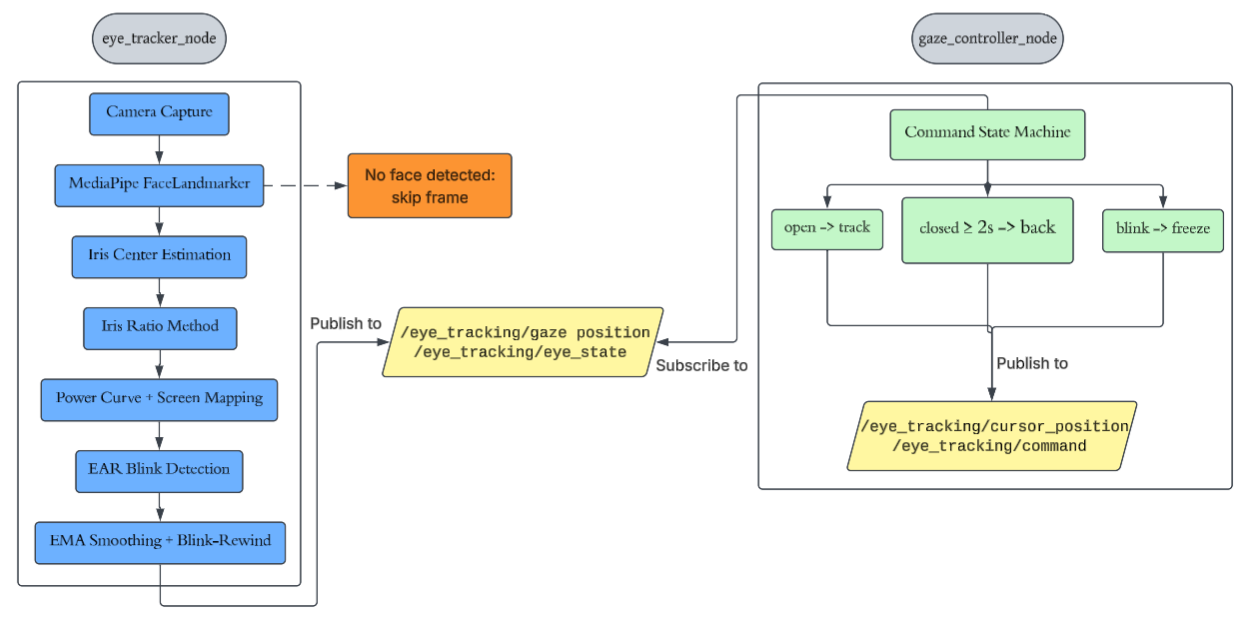
\includegraphics[width=475]{figures/ch08/the_diagram}
\caption{Sanad eye tracking pipeline: from camera capture to ROS~2 command dispatch.
Red dashed arrows indicate exception paths.}
\label{fig:gaze_pipeline}
\end{figure}



% ----------------------------------------------------------------
\section{System Performance and Observations}
% ----------------------------------------------------------------

At the current stage of the project, formal quantitative evaluation of gaze accuracy — such
as controlled angular error measurements or statistically significant success-rate trials —
has not yet been conducted. A structured user study with participants representing the target
population is planned as part of the testing phase. The observations
reported here reflect the development team's experience operating the system under realistic
indoor conditions during integration and functional testing.

\textbf{General responsiveness:} The pipeline runs at a stable 20--28 inference frames per
second on the Raspberry Pi~4 without any GPU acceleration. The end-to-end latency from eye
movement to cursor update is approximately 57--65~ms, which is imperceptible to the user
and well within the 200~ms threshold at which humans begin to notice interface lag.
The cursor feels immediate and natural to operate.

\textbf{Gaze tracking stability:} Under standard indoor lighting conditions, the
MediaPipe FaceLandmarker model tracks the iris consistently without dropout, and the EMA
smoothing ($\alpha = 0.30$) eliminates visible cursor jitter while preserving
responsiveness to deliberate gaze shifts. The blink-rewind buffer successfully prevents the
cursor from drifting downward during natural blinks, which was a noticeable artefact in
early testing before the buffer was introduced.

\textbf{Dwell activation reliability:} The edge-popup buttons activate reliably when gaze
is held intentionally at a screen edge. No false activations were observed during normal
reading or resting gaze within the central screen area, confirming that the 18\% edge-trigger
threshold effectively separates intentional peripheral gaze from passive content viewing.

\textbf{Eye-closure command:} The 2-second sustained closure threshold for back/confirm
commands proved comfortable in practice. Natural blinks (typically 150--400~ms in
duration) never triggered the command, and intentional closures were
consistently recognised without requiring excessive effort from the operator.

\textbf{Computational headroom:} CPU usage across both nodes remains within 30--45\% of a
single Pi~4 core, leaving the remaining processing capacity fully available for the
concurrent touchscreen interface, ROS~2 middleware, and other Sanad subsystems running on
the same board.

Formal accuracy benchmarking, including gaze-point error under varying lighting conditions and multi-session dwell success rates, remains as future work.

\section{Summary and Transition}
This chapter has detailed the webcam-based eye-gaze tracking pipeline, which enables hands-free system navigation and interaction. The next chapter, Chapter 9 (Mobile Application), extends control to the user's care network by detailing the cross-platform application designed for remote monitoring and diagnostics.

